\chapter{Introduction}
\addcontentsline{toc}{chapter}{Introduction}
\markboth{Introduction}{Introduction}
\label{chap:introduction}
%\minitoc

%%% Local Variables: 
%%% mode: latex
%%% TeX-master: "isae-report-template"
%%% End: 

\section{D3S, a leader in 3D CAD Analytics}

D3S, which stands for Data Science Softwares \& Services, specializes in delivering customized software solutions utilizing AI technologies. The company comprises a team of Data Scientists and Full Stack Developers with deep expertise in 3D CAD (Computer-Aided Design) Analytics and Natural Language Processing (NLP).  

Its state-of-the-art technologies are built on open-source libraries and supported by internal R\&D, enabling efficient data extraction through computer vision, Optical Character Recognition (OCR), and NLP. D3S also excels in deep learning applications such as 3D morpho analysis, metrics comparison, BoM (Bill of Materials) analytics, and time series processing. 

The company’s solutions are designed to provide scalable, adaptable, and secure business value for industries like aerospace and automotive.

\vspace{0.5cm}

I will be working with the 3D CAD Analytics team, where my focus will be on developing a 3D similarity model designed to compare CAD models solely based on their geometric properties.

\begin{figure}[]
    \centering
    
\includegraphics[width=0.3\columnwidth]{images/d3s_logo.png}
    \caption{D3S, Data Science Softwares \& Services}
    \label{fig:d3s_logo}
\end{figure}

\section{3D similarity model}

The goal is to automatically associate a given piece to similar other pieces, as depicted in \autoref{fig:similar-pieces}. This will make it possible to leverage the D3S dataset of industrial 3D models, in order to infer missing information, such as the name of a piece, its function, or its material.

\begin{figure}[]
    \centering
    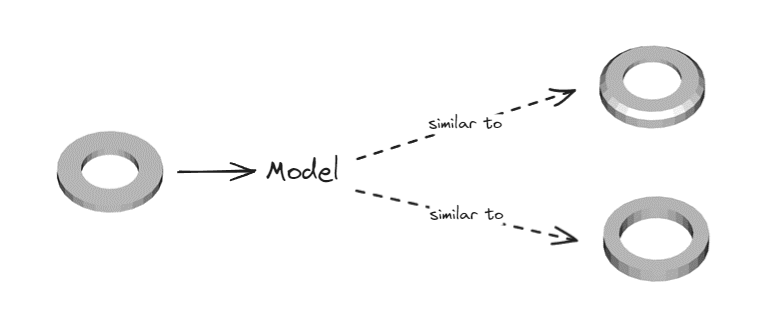
\includegraphics[width=0.8\columnwidth]{images/similar-pieces.png}
    \caption{Purpose of our similarity model}
    \label{fig:similar-pieces}
\end{figure}

In recent years, point cloud representations has become one of the research hotspots in the field of computer vision \cite{zhangDeepLearningbased3D2023}.
In our case, we can not directly train a powerful mesh classifier, because of a lack of clean labeled data and of the variety of the possible 3D models.
The most comprehensive dataset available consists of just 2,000 CAD models, with rather imprecise labeling. Examples of labels include coupling strap, shackle, and long beam. It is evident that there is a significant need for a more curated and accurate dataset in this area, which is really hard to obtain.

Given the recent success of self-supervised learning methods, more specifically contrastive learning \cite{radfordLearningTransferableVisual2021,yuPointBERTPretraining3D2022,liuOpenShapeScaling3D2023}, an innovative and promising approach has been proposed to tackle this problem.

The goal is to learn a representation of data such that similar instances are close together in the representation space, while dissimilar instances are far apart. To do so, a triplet loss, popularized by the FaceNet model \cite{schroffFaceNetUnifiedEmbedding2015}, will be used. Since we lack labeled data, we can't generate triplets directly as in \cite{schroffFaceNetUnifiedEmbedding2015}. Instead, a 'Tinder-like' application has been developped and used by the whole company to build our 'labeled' triplets database.

To summarize, the pipeline comprises the two main following steps:
\begin{enumerate}
    \item \textbf{Triplets collection}: Offline 'unlabeled' triplets are generated. Triplets are then labeled by the users of the app and stored in the database.
    \item \textbf{Model training}: An encoding model is trained on the labeled triplets. The model is then used to compute the similarity between two 3D models.
\end{enumerate}

\begin{figure}[]
    \centering
    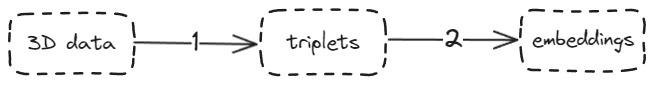
\includegraphics[width=0.8\columnwidth]{images/steps.png}
    \caption{Pipeline for building the model}   
    \label{fig:steps}
\end{figure}